\documentclass{article}
\usepackage[utf8]{inputenc}
\usepackage[hungarian]{babel}

\usepackage{amsmath}

\usepackage{lipsum}
\usepackage{graphicx} % for the includegrapichs
\usepackage{titling}

\usepackage{fancyhdr} % for the header on the first page
\usepackage{pdfpages} % to include pdf
\usepackage{structuralanalysis} % for the figures
\usepackage{multicol}
\usepackage{wasysym}
\usepackage{t1enc}
\usepackage{textcomp}
\usepackage[left=3cm,right=3cm,top=3.5cm,bottom=3.5cm,headsep=50pt]{geometry}

\begin{document}
	
	\begin{titlepage}
		\setlength{\headheight}{20pt}
		\lhead{
\includegraphics[height=1.5cm]{logo_mm.png}}
		\rhead{\large{\textbf{Végeselem módszer alapjai}}\\
			BMEGEMMAGMV}
		%\vspace{15cm}
		\title{\huge Kötelező házi feladat 1
		}
		\author{Tar Dániel\\GUTOY7}
		\date{\today}
		\maketitle
		\pagenumbering{gobble}
		\thispagestyle{fancy}
		
		\begin{figure}
			\begin{center}
				
\includegraphics[height=2cm]{logo_bme_kicsi.eps}
			\end{center}
		\end{figure}
		
	\end{titlepage}
	\newpage

	%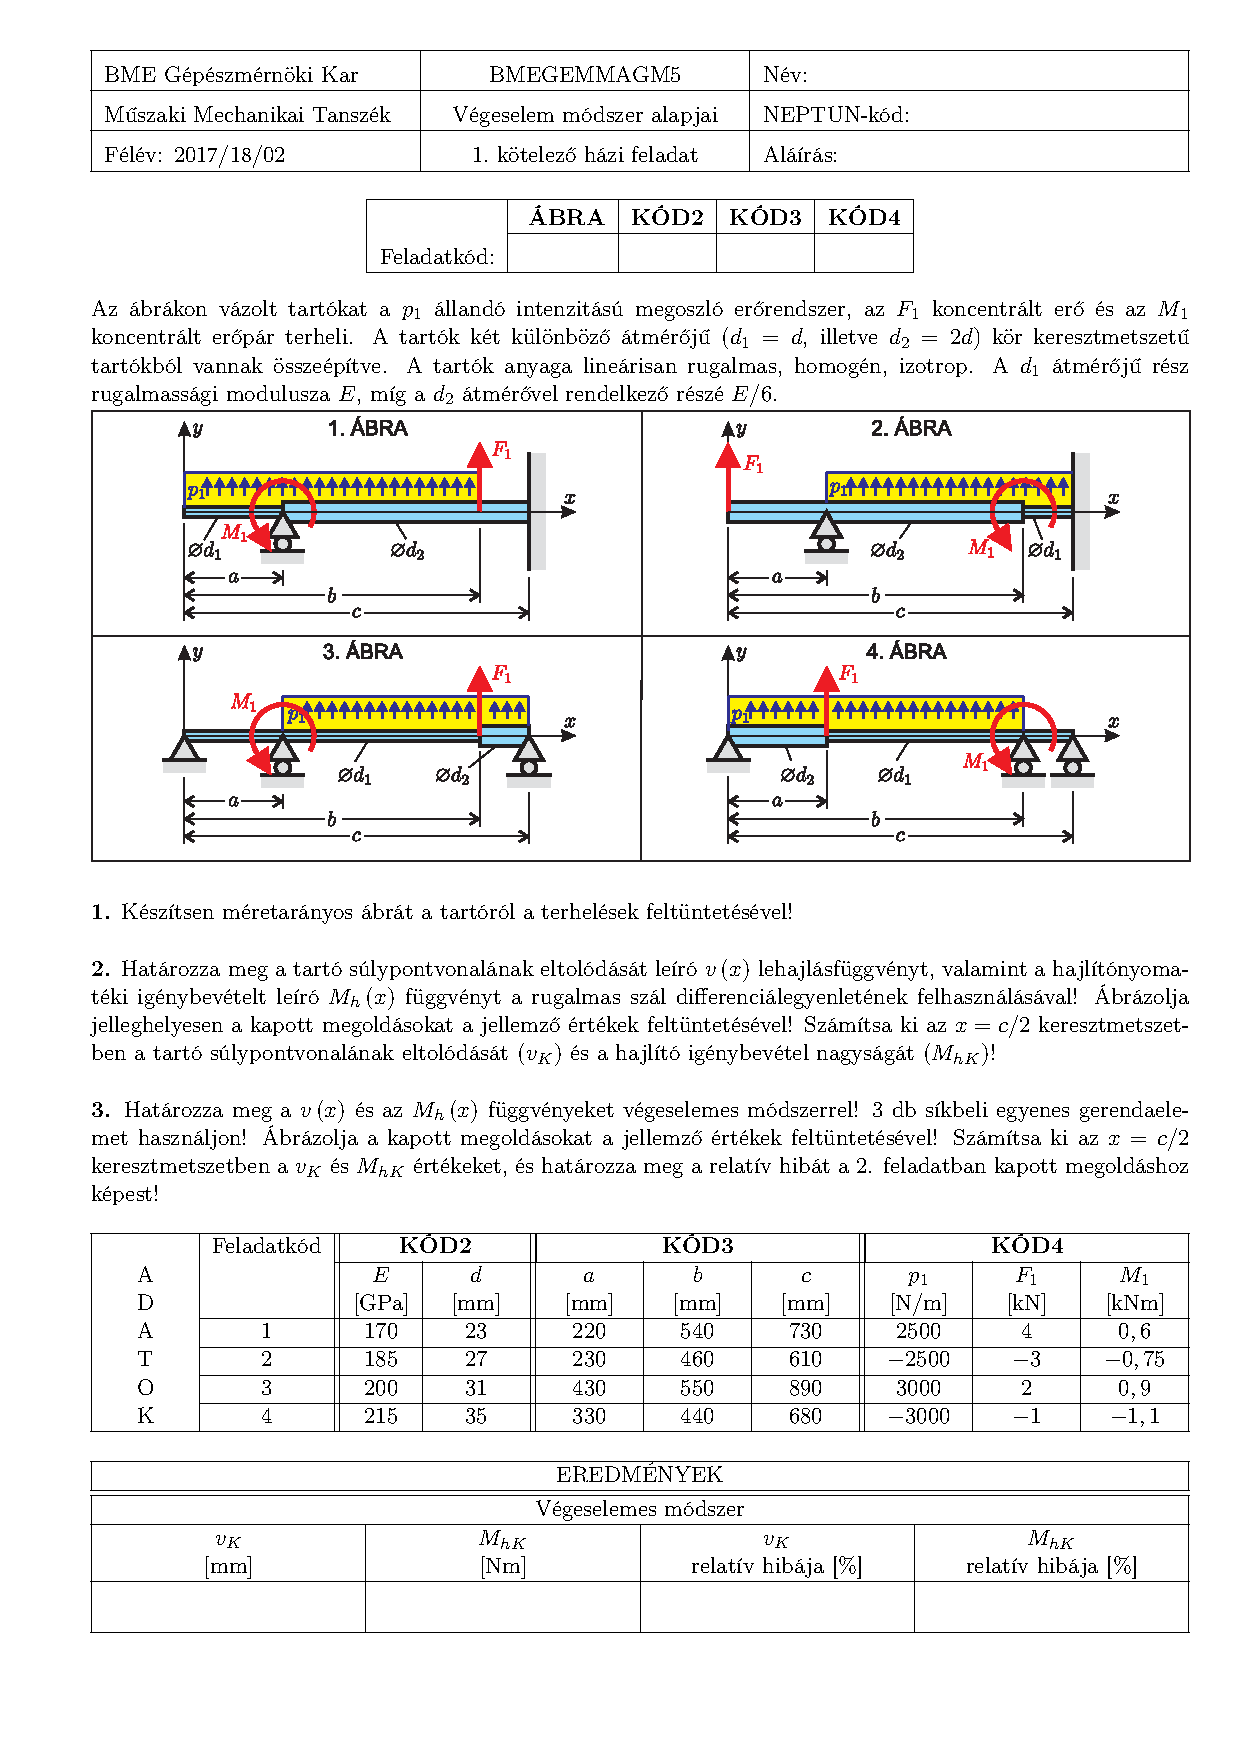
\includepdf{vemalaphf1.pdf}
	 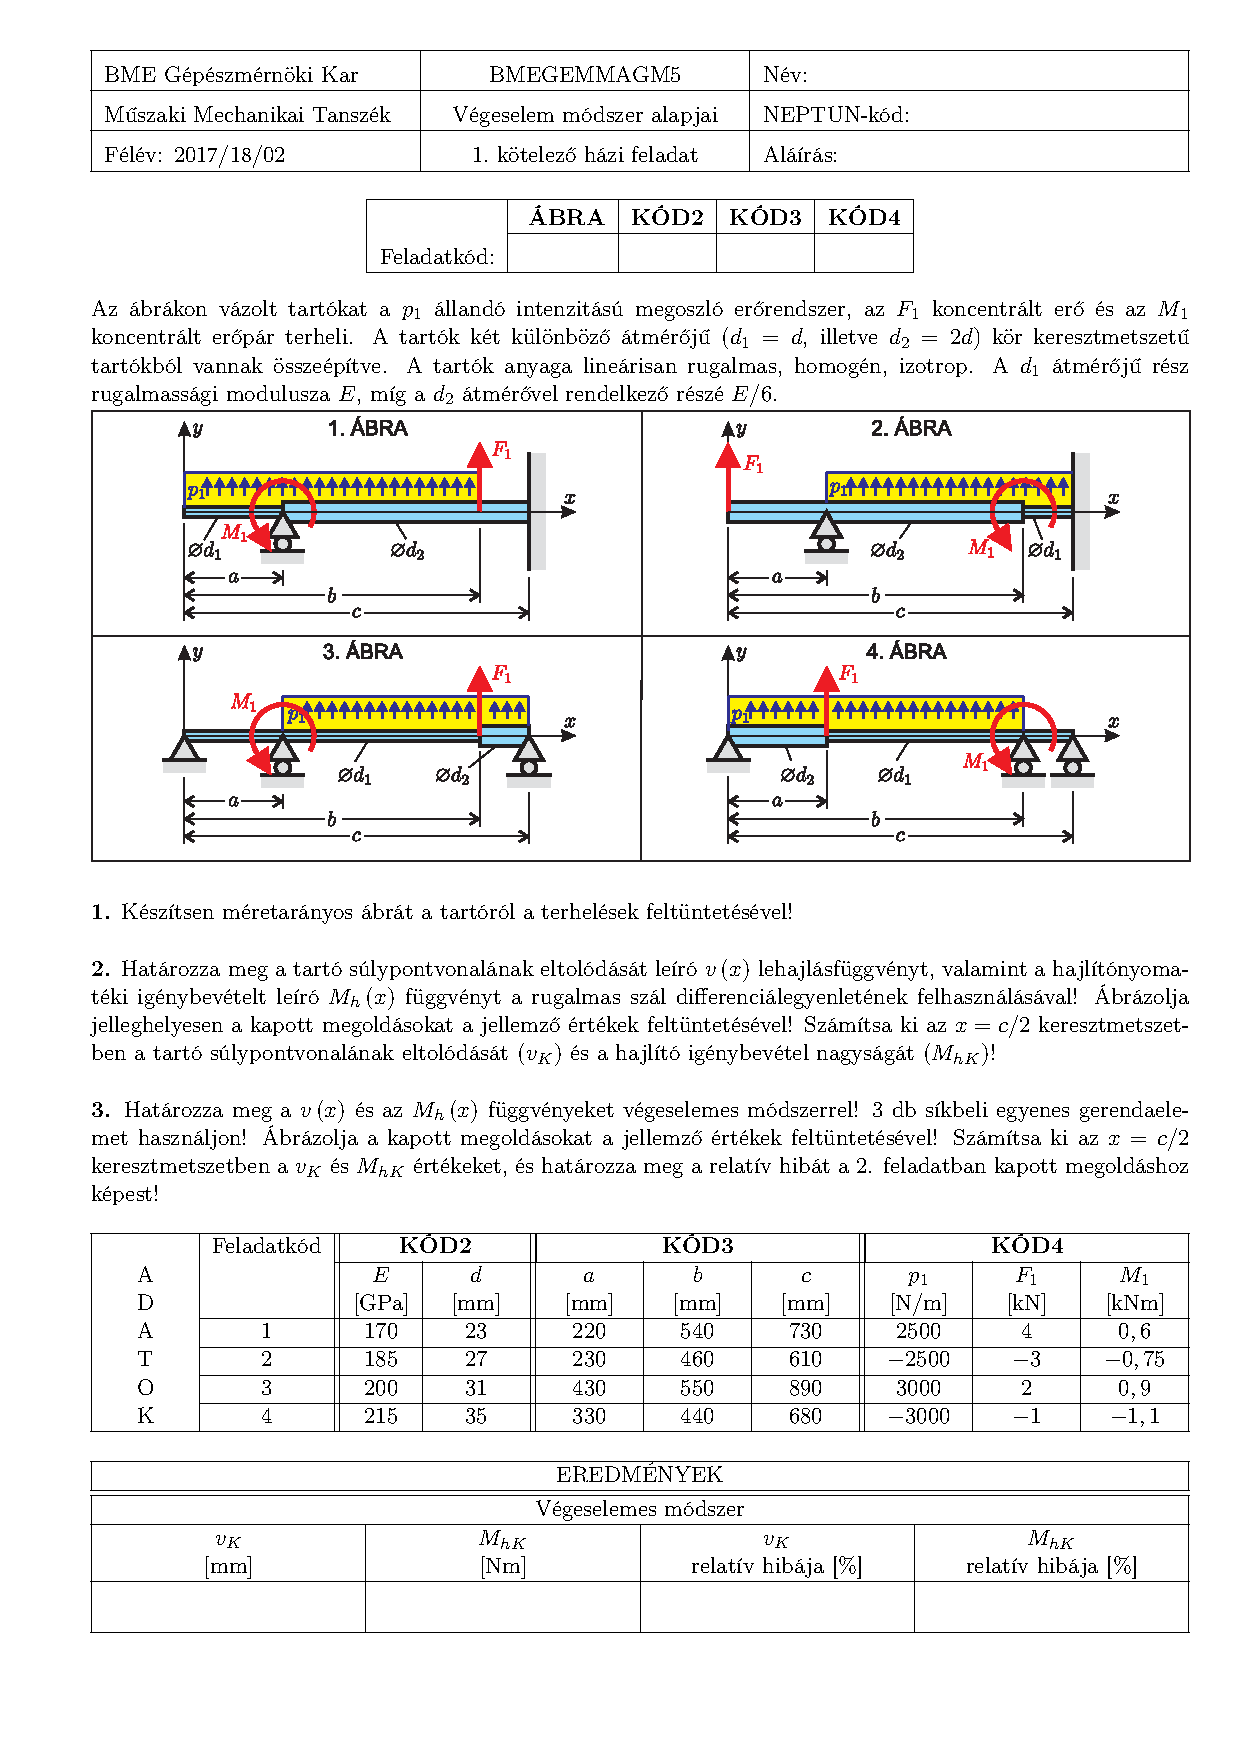
\includepdf[picturecommand*={
	    	\put(460,759){Tar Dániel}
	    	\put(460,740){GUTOY7}
	    	\put(280,677){2}
	    	\put(327,677){1}
	    	\put(370,677){2}
	    	\put(415,677){2}
	    	\put(116,63){0,8096}
	    	\put(238,63){652,5147}
	    	\put(369,63){-0,54}
	    	\put(490,63){-0,28}
	 }]{vemalaphf1.pdf}
	\newpage
	
	
	\setlength{\headheight}{0pt}
	\tableofcontents
	\newpage
	
	\pagenumbering{arabic}	
	\setcounter{page}{1}

	
	
	

	
	%\newpage
	%---------------------
	% 1.feladat
	%---------------------
	\section{Feladat}
	
		A házifeladat kód alapján az adatokat átszámolva $[N][m][Pa]$ alapra:
		\def\arraystretch{1.2}%
		\begin{table}[h!]
			\begin{center}
				\caption{Adatok}
				\label{tab:table1}
				\begin{tabular}{c|c|c|c|c|c|c|c|c|c} % <-- Alignments: 1st column left, 2nd middle and 3rd right, with vertical lines in between
					$E_1$  	&	$E_2$	& $d_{1}$ 	& $d_{2}$ & $a$ & $b$ & $c$ & $p_{1}$ & $F_{1}$ & $M_{1}$ \\
					$[Pa]$ 	&	$[Pa]$	& $[m]$ 	& $[m]$ & $[m]$ & $[m]$ & $[m]$ & $[N/m]$ & $[N]$ & $[Nm]$\\
					\hline
					$170\cdot10^9$ & $28,33\cdot10^9$ & $23\cdot10^{-3}$ & $46\cdot10^{-3}$ & $230\cdot10^{-3}$ & $460\cdot10^{-3}$ & $610\cdot10^{-3}$ & -2500 & -3000 & -750\\
				\end{tabular}
			\end{center}
		\end{table}\\[10pt]
		\def\arraystretch{1}%
		Az alapadatokból származtatott adatok (kereszmetszetek felületei, másodrendű nyomatékai):	
		\begin{equation}
		A_1=\frac{d_1^{2}\cdot\pi}{4}=4,1548 \cdot 10^{-4}~[m^{2}]
		\end{equation}
		\begin{equation}
		A_2=\frac{d_2^{2}\cdot\pi}{4}=16,619 \cdot 10^{-4}~[m^{2}]
		\end{equation}
		\begin{equation}
		I_{z1}=\frac{d_1^4\cdot\pi}{64}=1,3737 \cdot 10^{-8}~[m^{4}]
		\end{equation}
		\begin{equation}
		I_{z2}=\frac{d_2^4\cdot\pi}{64}=21,9787 \cdot 10^{-8}~[m^{4}]
		\end{equation}\\[10pt]
		A terheléseket arányosan és mindenhol a pozitív irányba vettem fel, hogy megegyezzen a feladatleírásban szereplő ábrával.
	
	%\newcommand{\newCommandName}{text to insert}
	\newcommand{\degy}{8}
	\newcommand{\dketto}{16}
	
	\begin{figure}[h!]
		\begin{center}
			\begin{tikzpicture}
			\scaling{.015};
			
			% x and y axis
			\draw[->] (0,0)--(10,0) node[right]{$x$};
			\draw[->] (0,0)--(0,3) node[above]{$y$};
			
			% auxiliary points
			\point{a}{0}{0};
			\point{b}{230}{0};
			\point{c}{460}{0};
			\point{d}{610}{0};
			\point{e}{0}{\dketto}; %only to see it works :D
			\point{f}{0}{-\dketto};
			\point{g}{460}{\dketto};
			\point{h}{460}{-\dketto};
			\point{i}{460}{\degy};
			\point{j}{460}{-\degy};
			\point{k}{610}{\degy};
			\point{l}{610}{-\degy};
			
			
			\point{a2}{0}{78};
			\point{b2}{230}{53};
			\point{c2}{450}{-\dketto};
			\point{d2}{610}{53};
			
			% stucture
			\beam{2}{e}{f};
			\beam{2}{e}{g};
			\beam{2}{f}{h};
			\beam{2}{g}{h};
			\beam{2}{i}{k};
			\beam{2}{j}{l};
			
			%\support{type}{insertion point}[rotation];
			\support{2}{b};
			\support{3}{d}[90];
			
			% loads
			% \load{type}{insertion point}[rotation][length or included angle][loaddistance];
			\load{1}{a2}[90][-1];
			\load{3}{c}[25][200][0.7];
			\lineload{2}{b2}{d2}[-0.83][-0.83];
			
			% dimensions
			\dimensioning{1}{a}{b}{-1.2}[$230~mm$];
			\dimensioning{1}{a}{c}{-2.2}[$460~mm$];
			\dimensioning{1}{a}{d}{-3.2}[$610~mm$];
			%\dimensioning{2}{f}{e}{-1}[$54$];
			
			
			
			\notation{1}{a}{$A$}[left];
			\notation{1}{b}{$B$}[above left=2.5mm];
			\notation{1}{c}{$C$}[below right=2.5mm];
			\notation{1}{d}{$D$}[above right=2.5mm];
			
			\notation{1}{a2}{$F_{1}$}[right];
			\notation{1}{b2}{$p_{1}$}[below right];
			\notation{1}{c2}{$M_{1}$}[below=1mm];
			
			
			\end{tikzpicture}
		\end{center}	
		\caption{Méretarányos ábra és a terhelések}
	\end{figure}


	\begin{flushleft}
		A rekcióerőket az pozitív x, y, és z irányoknak megfelelően vettem fel.
	\end{flushleft}
	
	\newpage
	%---------------------
	% 2.feladat
	%---------------------
	\section{Feladat - Rugalmas szál differenciálegyenlete}
	%\subsection{Hajlítónyomatéki függvények}
		A rugalmas szál diffrenciálegyenletéhez a hajlítónyomatéki függvények felírása szükséges. A tartót 3 részre osztottam és mind a három tartományra felírhatam a hajlítónyomatéki függvényeket:
		\def\arraystretch{2}
		\begin{table}[h!]
			\begin{center}
				\caption{Hajlítonyomatéki függvények}
				\label{tab:table2}
				\begin{tabular}{l|r} % <-- Alignments: 1st column left, 2nd middle and 3rd right, with vertical lines in between
					${M_h}_1=\ -F_1\cdot x$ & $0\le x\le a$\\
					${M_h}_2=\ -F_1\cdot x-F_B\cdot\left(x-a\right)-p_1\cdot\frac{\left(x-a\right)^2}{2}$ & $a\le x\le b$\\
					${M_h}_3=\ -F_1\cdot x-F_B\cdot\left(x-a\right)-p_1\cdot\frac{\left(x-a\right)^2}{2}+M_1$ & $b\le x\le c$
				\end{tabular}
			\end{center}
		\end{table}\\[10pt]
		\def\arraystretch{1}%
		A rugalmas szál differenciálegyenlete a három tarományra:
		\begin{equation}
			v_1^{\prime\prime}\left[x\right]=\frac{Mh_1\left[x\right]}{I_{z2}\cdot E_2}
		\end{equation}
		\begin{equation}
			v_2^{\prime\prime}\left[x\right]=\frac{Mh_2\left[x\right]}{I_{z2}\cdot E_2}
		\end{equation}
		\begin{equation}
			v_3^{\prime\prime}\left[x\right]=\frac{Mh_3\left[x\right]}{I_{z1}\cdot E_1}
		\end{equation}\\[10pt]
		A differenciálegyenletek megoldásához illesztési feltételeket, kényszerfelételeket, illetve statikai egyensúlyt leíró egyenleteket is fel kell írni.
		
		Illesztési feltételek:
		\begin{center}
			$\phi_1(a)=\phi_2(a)$\\
			$\phi_2(b)=\phi_3(b)$\\
			$v_1(a)=v_2(a)$\\
			$v_2(b)=v_3(b)$\\
		\end{center}
		
		Kényszerek: 
		\begin{center}
			$v_1(a)=0$\\
			$v_3(c)=0$\\
			$\phi_3(c)=0$\\
		\end{center}
	
		Egyensúlyi egyenletek:
		\begin{equation}
			\sum{F_x=0} :\ \ \ F_{Dx}=0
		\end{equation}
		\begin{equation}
			\sum{F_y=0} :\ \ \ F_1+F_{By}+p_1\cdot(c-a)+F_{Dy}=0
		\end{equation}
		\begin{equation}
			\sum{M_D=0} :\ \ \ -F_1\cdot c-F_{By}\cdot(c-a)-p_1\cdot\frac{(c-a)^2}{2}+M_1+M_D=0
		\end{equation}\\[10pt]		
		A rugalmas szál differenciálegyenleteiből a lehajlásfüggvényeket kétszeres integrálással kaphatjuk meg. Az integrálások miatt 6[db] ismeretlen értékű integrálási konstans jelenik meg. Ezen hat ismeretlenen kívül, ismeretlenek még a reakcióerők $(F_{By}, F_{Dx}, F_{Dy}, M_{D})$.
		Így egy tíz ismeretlenes egyenletrendszer áll elő, amelyekhez 10 peremfeltételt határoztunk meg. Ennek megfelelően az egyenletrendszerből az összes ismeretlen meghatározható.
		
		A számolt értékek közül a reakcióerők:
		\begin{center}
			$F_B = 3639,0266~[N]$\\
			$F_{Dx} = 0~[N]$\\
			$F_{Dy} = 310,9734~[N]$\\
			$M_D = 122,3301~[Nm]$
		\end{center}
		Az érékeket visszahelyettesítve a lehajlás-$^{\ref{diff_lehaj}}$ és hajlítónyomatéki$^{\ref{diff_nyom}}$ függvényekbe, azokat ábrázolva: 
		\begin{figure}[h!]
			\begin{center}
				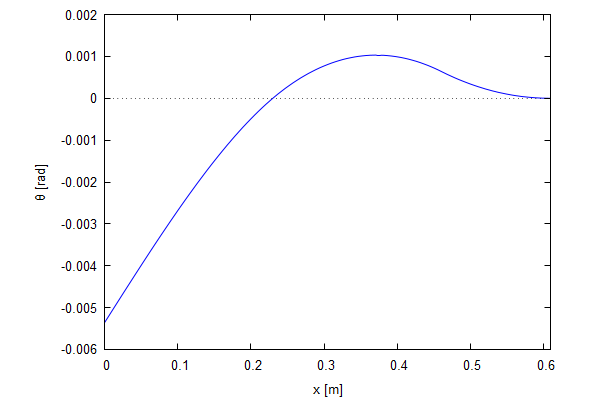
\includegraphics[height=10cm]{images/diff_lehaj}
			\end{center}
			\caption{Lehajásfüggvény}
			\label{diff_lehaj}
		\end{figure}
	\newpage
		\begin{figure}[h!]
			\begin{center}
				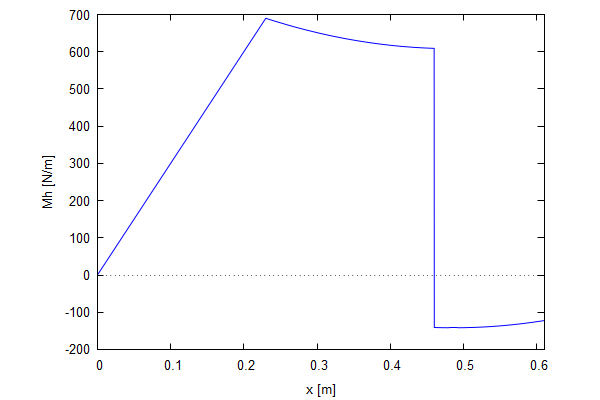
\includegraphics[height=10cm]{images/diff_nyomatek}
			\end{center}
			\caption{Hajlítónyomatéki függvény}
			\label{diff_nyom}
		\end{figure}
	
	%---------------------
	% 3.feladat
	%---------------------
	\section{Feladat - Végeselemes megoldás}
	\subsection{A reakcióerők és az elmozdulásvektor meghatározása}
		A feladat szövege alapján a végeselemes modell:
		\newcommand{\sugar}{2}
		\newcommand{\ab}{230}
		\newcommand{\ac}{460}
		\newcommand{\ad}{610}
		\newcommand{\adv}{610}
		\newcommand{\advv}{610}
		\begin{figure}[h!]		
			\begin{center}	
				\begin{tikzpicture}
				\scaling{.022};
				% auxiliary points
				\point{a}{0}{0};
				\point{b}{\ab}{0};
				\point{b1}{\ab*2}{0};
				\point{c}{\ac}{0};
				\point{d}{\ad}{0};
				\point{d2}{210}{35};
				
				\beam{2}{a}{b};
				\beam{2}{b}{c};
				\beam{2}{c}{d};
				
				\support{2}{b};
				\support{3}{d}[90];
				
				\hinge{1}{a};
				\hinge{1}{b};
				\hinge{1}{c};
				
				\notation{1}{a}{$(1)$}[above];
				\notation{1}{b}{$(2)$}[above];
				\notation{1}{c}{$(3)$}[above];
				\notation{1}{d}{$(4)$}[above left];
				
				\notation{5}{a}{b}[$I, E, A$][.5][below];
				\notation{5}{b}{c}[$I, E, A$][.5][below];
				\notation{5}{c}{d}[$I, E, A$][.5][below];
				
				\notation{4}{a}{b}[1]
				\notation{4}{b}{c}[2]
				\notation{4}{c}{d}[3] 
				\end{tikzpicture}
			\end{center}	
			\caption{Végeselemes modell}
		\end{figure}\\[10pt]	
		Elemi merevségi mátrix:
		\begin{equation}
		K_{e,4\times4}= \frac{I_{z} \cdot E}{L^3}  
			\begin{bmatrix}
			12&6L&-12&6L\\
			6L&4L^2&-6L&2L^2\\
			-12&-6L&12&-6L\\
			6L&2L^2&-6L&4L^2\\
			\end{bmatrix}
			=\begin{bmatrix}
			K_{11} &K_{12} \\
			K_{21} &K_{22} \\
			\end{bmatrix}
		\end{equation}\\[10pt]
		A 3[db] egyenes gerendaelem elemi merevségi mátrixait elhelyezzük a globális merevségi mátrixban a hozzájuk tarozó szabadsági fok összerendelések alapján.\\[10pt]
		Globális merevségi mátrix:
		\begin{equation}
		K_{G,8\times8}=
		\begin{bmatrix}
		K_{11}^{(1)} & K_{12}^{(1)}              & 0            			    & 0            \\
		K_{21}^{(1)} & K_{22}^{(1)}+K_{11}^{(2)} & K_{12}^{(2)}  			    & 0            \\
		0            & K_{21}^{(2)}              & K_{22}^{(2)} + K_{11}^{(3)}  & K_{12}^{(3)} \\
		0            & 0						 & K_{21}^{(3)} 					& K_{22}^{(3)} \\
		\end{bmatrix}
		\end{equation}
		Ahol az általános elmozdulás és tehervektor:
		\begin{equation}
			{\underline{U}}^T=[V_1\ \ \Theta_1\ \ V_2\ \ \Theta_2\ \ V_3\ \ \Theta_3\ \ V_4\ \ \Theta_4]
		\end{equation}
		\begin{equation}
			{\underline{F}}^T=[f_1\ \ m_1\ \ f_2\ \ m_2\ \ f_3\ \ m_3\ \ f_4\ \ m_4] 
		\end{equation}
		A tehervektor a koncentrált erők és megoszló terhelések összegeként írható fel. A megoszló erőt a két rúdra külön felírva:
		\def\arraystretch{2}
		\begin{table}[h!]
			\begin{center}
				\caption{Tehervektor részei}
				\label{tab:table3}
				\begin{tabular}{l c r} % <-- Alignments: 1st column left, 2nd middle and 3rd right, with vertical lines in between
					$F_{konc}=
					\begin{bmatrix}
						F_{1}    \\
						0\\
						0\\
						0\\
						0\\
						M_{1} \\
						0\\
						0\\
					\end{bmatrix} [SI]$ \ \ \ \ \ \ & 
					$F_{1_{rud_2}}= p_1 \cdot \frac{L_2}{12}
					\begin{bmatrix}
						0\\
						0\\
						6\\
						L_{2} \\
						6\\
						-L_{2} \\
						0\\
						0\\
						\end{bmatrix} [SI]$  \ \ \ \ \ \ & 
					$F_{1_{rud_3}}= p_1 \cdot \frac{L_3}{12}
					\begin{bmatrix}
						0\\
						0\\
						0\\
						0\\
						6\\
						L_{3} \\
						6\\
						-L_{3} \\
					\end{bmatrix} [SI]$
				\end{tabular}
			\end{center}
		\end{table}\\[10pt]
		\def\arraystretch{1}%
		Az elmozdulásvektor megkötött paraméterei alapján kondenzáljuk a globális merevségi mátrixot úgy, hogy a merevségi mátrix oszlopait és sorait töröljük ott ahol az elmozdulásvektor nulla.
		
		A kondenzált merevségi mátrix:
		\begin{equation}
		K_{G,K,5\times5}=
		\begin{bmatrix}
		K_{G_{11}}	 & K_{G_{12}}	 & K_{G_{14}} & K_{G_{15}}	 & K_{G_{16}}  \\
		K_{G_{21}}	 & K_{G_{22}}	 & K_{G_{24}} & K_{G_{25}}	 & K_{G_{26}}  \\
		K_{G_{41}}	 & K_{G_{42}}	 & K_{G_{44}} & K_{G_{45}}	 & K_{G_{46}}  \\
		K_{G_{51}}	 & K_{G_{52}}	 & K_{G_{54}} & K_{G_{55}}	 & K_{G_{56}}  \\
		K_{G_{61}}	 & K_{G_{62}}	 & K_{G_{64}} & K_{G_{65}}	 & K_{G_{66}}  \\
		\end{bmatrix}
		\end{equation}
		
		A kondenzált elmozdulásvektor:
		\begin{equation}
			\textbf{U}_{kond}=
			\begin{bmatrix}
			V_{1}    \\
			\Theta_{1} \\
			\Theta_{2} \\
			V_{3}    \\
			\Theta_{3} \\
			\end{bmatrix} [SI]
		\end{equation}\\[10pt]
		Az így alkotott $\textbf{K}_{kond}\cdot\textbf{U}_{kond}=\textbf{F}_{kond}$ egyenletrendszer megoldásával az elmozdulásvektor:
		\begin{equation}
			\textbf{U}=
			\begin{bmatrix}-0.0053\\
			0.0276\\
			0\\
			0.0148\\
			6.4165 {{10}^{-4}}\\
			-0.0088\\
			0\\
			0
			\end{bmatrix} [SI]
		\end{equation}
		A tehervektort pedig az elmozdulásvektor visszahelyettesítésével:
		\begin{equation}
			\textbf{F}=
			\begin{bmatrix}-3000\\
			0\\
			3351.5266\\
			-11.0208\\
			-475\\
			-743.6667\\
			123.4734\\
			127.0176
			\end{bmatrix} [SI]
		\end{equation}
		A tehervektor komponenseiből kiolvashatóak a reakcióerők:
		\begin{equation}
			\textbf{F}_{reak}=
			\begin{bmatrix}
			0\\
			0\\
			3639.026588296437\\
			0\\
			0\\
			0\\
			310.9734117035641\\
			122.3301035526437
			\end{bmatrix} [SI]
		\end{equation}
		A végeselemes megoldás útján kapott eredmények szinte teljesen megegyeznek a rugalmas szál differenciál egyenletével számolt eredményekkel.
	\subsection{Lehajlási és nyomatéki függvény meghatározása}
		Harmadfokú polinommal történik az elmozdulásmező interpolációja.
		\begin{equation}
			w(x)=a_0+a_1\xi+a_2\xi^2+a_3\xi^3
		\end{equation}
		Amely egyenletben a konstansok meghatározásához peremfeltételeket írhatunk fel:
	    \begin{center}
	    	$w\left(x=0\right)=v_i$\\
	    	$\frac{dw\left(x\right)}{dx}\left(x=0\right)=\mathrm{\Theta}_i$\\
	    	$w\left(x=L\right)=v_j$\\
	    	$\frac{dw\left(x\right)}{dx}\left(x=L\right)=\mathrm{\Theta}_j$\\	
	    \end{center}
		A lokális mátrixot felírva az egyenletrendszer paramétereit behelyettesítve megkaphatjuk az alábbi vektort:
		\begin{equation}
			\begin{bmatrix}2 {{\xi}^{3}}-3 {{\xi}^{2}}+1\\
			L\, {{\xi}^{3}}-2 L\, {{\xi}^{2}}+L \xi\\
			3 {{\xi}^{2}}-2 {{\xi}^{3}}\\
			L\, {{\xi}^{3}}-L\, {{\xi}^{2}}\end{bmatrix}
		\end{equation}
		
	\subsubsection{A lokális vektorból globálisba történő átalakítás}	
		A végeselemes módszernél a gerendaelemek lehajlását az alábbbi egyenlettel határozhatjuk meg:
		egyenlet...
		ahol i = 1,2,3.
		
		A kszi lokális koordinátából az x globális koordinátába való átállás:
		keplet...
		
		Ez alapján már meghatározhatók a lehajlásfüggvények az egyes gerendaelemekre a globális koordinátarendszerben.
		Ha ezeket a függvényeket 2x deriváljuk x szerint, akkor keresztmetszet nyomatékfüggvényeit kapjuk:
		függvények...
		
		A rugalmas szál differenciálegyenletével és a VEM-es módszerrel kapott lehajlásfüggvények közel megegyeznek, annak ellenére hogy a hajlító nyomatéki függvény csak lináris részelemeket tartalmaz.
		
		Lehajlás- és nyomatéki függvény:
		lehajlási, nyomatéki + ábra
	\subsection{Relatív hiba számítása}	
		A vk és Mhk értékek az x=c/2 helyen:
		\begin{itemize}
			\item Rugalmas szál differenciálegyenletével kapott értékek
			\begin{equation}
				salala = asla
			\end{equation}
			\item VEM-es módszerrel kapott értékek
			\begin{equation}
			salala = asla
			\end{equation}
		\end{itemize}
		
		A rugalmas szál diff. egyenletére vonatkoztatott relatív hiba:
		képletek...
		
		Konklúzió melyik minel nagyobb hány százalékkal..
		
		
		
	
	

\end{document}
